
\documentclass[a4paper,11pt]{article}

\usepackage{amsmath,amssymb,amsfonts,amsthm}    % Typical maths resource packages
\usepackage{graphicx}                           % Packages to allow inclusion of graphics
\usepackage{hyperref}                           % For creating hyperlinks in cross references
\usepackage[authoryear]{natbib}                 % literature reference style
\usepackage[bf]{caption2}
\usepackage{wrapfig,lipsum,booktabs}
\usepackage{subfig}

\usepackage[scaled=0.92]{helvet}
\renewcommand{\familydefault}{\sfdefault}
\fontfamily{phv}\selectfont

% -------------------------------
% --- some layout definitions ---
% -------------------------------

% define topline
\usepackage[automark]{scrpage2}
%\pagestyle{scrheadings}
%\automark{section}
%\clearscrheadings
%\ohead{\headmark}

% define citation style
\bibliographystyle{ieeetr}
\setcitestyle{square}

% define page size, margin size
\setlength{\headheight}{1.1\baselineskip}
\voffset=-2cm
\hoffset=-3cm
\textheight24cm
\textwidth15.5cm
\topmargin1cm
\oddsidemargin3cm
\evensidemargin3cm

% define line line spacing = 1.5
\renewcommand{\baselinestretch}{1.5}

% define second level for `itemizing'
\renewcommand{\labelitemii}{-}




% --------------------------------------
% --------------------------------------
% --------------------------------------
% --- the structure the tex document ---
% ---  (this our recommendation) -------
% frontmatter:
%   - titlepage (mandatory),
%   - acknowledgement,
%   - abstract,
%   - table of contents (mandatory),
%   - list of abbreviations (not mandatory),
%   - list of figures (not mandatory),
%   - list of tables  (not mandatory) .
%
% body of the thesis (the structure of the thesis body is not mandatory, but the list of literature is mandatory):
%   - introduction,
%   - methods,
%   - data,
%   - results,
%   - conclusion,
%   - literature (mandatory),
%   - appendix (figures, tables).
%
% last page:
%   - declaration of authorship (mandatory).
% --------------------------------------
% --------------------------------------
% --------------------------------------

\begin{document}

% -------------------------------
% --- frontmatter: Title page ---
% -------------------------------
\thispagestyle{empty}
\begin{center}

    {}\vspace{4cm}

    {\Large{\bf Master's Thesis}} \vspace{6cm}

    {\Large{\bf Implementation and Comparative Assessment of Diagnostic Cancer Gene Panels in the Molecular Pathology Laboratory}} \vspace{5cm}

    {\normalsize University of Luxembourg \\
    Faculty of Science, Communication and Technology
    } \vspace{1cm}

    {\normalsize Master in Integrated Systems Biology
    } \vspace{2cm}

    {\normalsize by \\\vspace{1cm}
    {\bf Ben Flies} \\
    (010081174D)} \vspace{1cm}

\end{center}




% ------------------------------------
% --- frontmatter: Acknowledgement ---
% ------------------------------------
%\newpage
%\pagestyle{plain}
%\pagenumbering{roman}   % define page number in roman style
%\setcounter{page}{1}    % start page numbering
%\section*{Acknowledgement}

I would like to thank




% -----------------------------
% --- frontmatter: Abstract ---
% -----------------------------
\newpage
\section*{Abstract}

This is the template for a thesis at the Chair of Econometrics of
Humboldt--Universit\"at zu Berlin. A popular approach to write a
thesis or a paper is the IMRAD method (Introduction, Methods,
Results and Discussion). This approach is not mandatory! You can
find more information about formal requirements in the booklet
`Hinweise zur Gestaltung der \"au\ss eren Form von Diplomarbeiten'
which is available in the office of studies.\\

The abstract should not be longer than a paragraph of around 10 to
15 lines (or about 150 words). The abstract should contain a
concise description of the econometric/economic problem you
analyse and of your results. This allows the busy reader to obtain
quickly a clear idea of the thesis content.

\pagenumbering{gobble}



% -----------------------------
% --- frontmatter: Contents ---
% -----------------------------
\newpage
\tableofcontents
\clearpage
\pagenumbering{gobble}


% ----------------------------------------------------
% --- frontmatter: List of Figures (not mandatory) ---
% ----------------------------------------------------
\newpage
\renewcommand{\thepage}{\roman{page}}% Arabic page numbers
\setcounter{page}{1}
\addcontentsline{toc}{section}{List of Abbreviations}
\ohead[]{LIST OF ABBREVIATIONS}
\section*{List of Abbreviations}

\begin{table}[htbp]
\begin{tabular}{p{1cm} p{6.5cm} | p{1cm} p{6.5cm}}
    NGS     &  Next Generation Sequencing   & LNS     &  Laboratoire National de Sante  \\
    SGMB     &  Service of Genetics and Molecular Biology          & TST15     &  Illumina TruSight Tumor 15
\end{tabular}
\end{table}




% ----------------------------------------------------
% --- frontmatter: List of Figures (not mandatory) ---
% ----------------------------------------------------
\newpage
\addcontentsline{toc}{section}{List of Figures}
\ohead[]{\rightmark}
\listoffigures



% ---------------------------------------------------
% --- frontmatter: List of Tables (not mandatory) ---
% ---------------------------------------------------
\newpage
\addcontentsline{toc}{section}{List of Tables}
\listoftables



% -------------------------------
% --- main body of the thesis ---
% -------------------------------
\newpage
\pagestyle{plain}
\setcounter{page}{1}    % start page numbering anew
\pagenumbering{arabic}  % page numbers in arabic style


\section{Introduction}

\begin{itemize}

\item What is the subject of the study? Describe the
economic/econometric problem.

-> Implementation of Cancer Gene Panels & Variant Calling Algorithms

\item What is the purpose of the study (working hypothesis)?

-> Check whether one of them is better than the others.
-> Study effect of FFPE

\item What do we already know about the subject (literature
review)? Use citations: { \cite{mutect:2013} shows that...
Alternative Forms of the Wald test are considered
\citep{Breusch&Schmidt:88}.}

\item What is the innovation of the study?

-> relatively rare technique in diagnostics, but has many advantages

\item Provide an overview of your results.


\end{itemize}

>>> Internship Report

The accumulation of DNA mutations is a characteristic of tumors. Mutations in a cell’s genetic material enable the so-called cancer hallmarks, which include, amongst others, capabilities as activating invasion and metastasis, enabling replicative immortality, sustaining proliferative signaling or evading growth suppressors. Classical anti-cancer treatments are tailored for the „average patient“ and not for the individual. Traditional cytotoxic chemotherapeutic drugs, for instance, are unspecific and have numerous adverse effects [1]: they attack rapidly dividing cells and make no difference between healthy and cancer cells. For a long time, there was no possibility to predict the success of a patient’s cancer treatment. In consequence, the treating clinician had no way to personalize the treatment to the individual patient.

The completion of the human genome project and technical advances in the field of genetics, in combination with advanced computer performance, enabled geneticists and pharmacologists to adopt the personalization of cancer diagnostics and treatment. In oncology, the customized healthcare approach is designed to the individual patient by taking into account the genetic information from a patient’s tumor biopsy. Targeting proteins that give cancer cells a proliferative advantage, instead of simply using cytotoxic agents, allows a more specific treatment and might decrease treatment-associated side-effects. In the past years, the Food and Drug Administration (FDA, USA) has approved several drugs that specifically target proteins needed for cancerogenesis [2]. Many of these drugs are now competent treatments for several common cancers. In many patients, however, these agents might lack any efficiency: cancers are known to be highly heterogenous and mutations in some subpopulations of cancer cells make them resistant to the treatment [3]. Identifying these mutations is thereby an utmost necessity for tailoring a targeted and efficient cancer therapy. Amongst the many mutation detection techniques, Next Generation Sequencing (NGS) constitutes the most powerful method and allows deep insights into the underlying causes of diseases.



>>> Next-Generation Sequencing: Methodology and Application
Nucleic acid sequencing is a method for determining the exact order of nucleotides present in a given DNA or RNA molecule. In the past decade, the use of nucleic acid sequencing has increased exponentially as the ability to sequence has become accessible to research and clinical labs all over the world. The first major foray into DNA sequencing was the Human Genome Project, a %$3 billion, 13-year-long endeavor, completed in 2003. The Human Genome Project was accomplished with first-generation sequencing, known as Sanger sequencing. Sanger sequencing (the chain-termination method), developed in 1975 by Edward Sanger, was considered the gold standard for nucleic acid sequencing for the subsequent two and a half decades (Sanger et al., 1977).

Since completion of the first human genome sequence, demand for cheaper and faster sequencing methods has increased greatly. This demand has driven the development of second-generation sequencing methods, or next-generation sequencing (NGS). NGS platforms perform massively parallel sequencing, during which millions of fragments of DNA from a single sample are sequenced in unison. Massively parallel sequencing technology facilitates high-throughput sequencing, which allows an entire genome to be sequenced in less than one day. In the past decade, several NGS platforms have been developed that provide low-cost, high-throughput sequencing. Here we highlight two of the most commonly used platforms in research and clinical labs today: the LifeTechnologies Ion Torrent Personal Genome Machine (PGM) and the Illumina MiSeq. The creation of these and other NGS platforms has made sequencing accessible to more labs, rapidly increasing the amount of research and clinical diagnostics being performed with nucleic acid sequencing.

>>> Clinical Actionability Enhanced through Deep Targeted Sequencing of Solid Tumors
Next generation sequencing can facilitate personalized cancer therapy approaches by identifying actionable somatic events in tumor samples (1). Furthermore, high-quality sequencing data can reveal associations with sensitivity or resistance that can inform the development and implementation of targeted therapeutics and, in particular, aid in the design of future trials to validate findings and actionability. Critical alterations include mutations [single nucleotide variations (SNVs)14 and insertions and deletions (indels)], copy number variations (CNVs), and rearrangements that can potentially predict response and resistance to targeted agents. Whole genome sequencing (WGS) and whole exome sequencing (WES) allow the detection of SNVs, indels, CNVs, and rearrangements. However, the relatively low coverage of WGS and WES, as currently implemented in most of the sequencing laboratories (100–250×), may have limited ability to cost-effectively detect aberrations that are present in a subpopulation of tumor cells while identifying a myriad of aberrations of unknown clinical significance (2). Somatic aberrations present at low allele frequencies across different types of tumors (3, 4) can potentially impact patient prognosis or response (5) and thus are important to detect reliably. Targeted sequencing to a depth that allows detection of relatively low mutant allele frequency (MAF) may represent an alternative or a complement to WGS and WES to detect clinically relevant alterations. Additionally, in most clinical and research settings, the amount of DNA that can be isolated from tumor samples is limited and the DNA is often damaged owing to fixation and storage procedures such as those used with formalin-fixed paraffin-embedded (FFPE) samples. Therefore a multiplexed targeted platform that can generate reliable data with high sensitivity from limited amounts of DNA from FFPE samples is needed. Several targeted sequencing panels have been successfully implemented (6, 7). However, the details of a platform's design and parameterization will influence the precision and reliability of the molecular profiling results, impacting both translational research and clinical decision-making. Thus, it is of great value to explore multiple potential solutions in a real patient care environment until a community-wide solution is established, validated, and well accepted.

1: Roychowdhury S, Iyer MK, Robinson DR, Lonigro RJ, Wu YM, Cao X, et al. Personalized oncology through integrative high-throughput sequencing: a pilot study. Sci Transl Med 2011;3:111ra21.
5: Zhao BY, Pritchard JR, Lauffenburger DA, Hemann MT. Addressing genetic tumor heterogeneity through computationally predictive combination therapy. Cancer Discov 2014;4:166–74.
6: Wagle N, Berger MF, Davis MJ, Blumenstiel B, Defelice M, Pochanard P, et al. High-throughput detection of actionable genomic alterations in clinical tumor samples by targeted, massively parallel sequencing. Cancer Discov 2012;2:82–93.
7: Frampton GM, Fichtenholtz A, Otto GA, Wang K, Downing SR, He J, et al. Development and validation of a clinical cancer genomic profiling test based on massively parallel DNA sequencing. Nat Biotechnol 2013;31:1023–31.

>>> Next-generation sequencing-based multi-gene mutation profiling of solid tumors using fine needle aspiration samples: promises and challenges for routine clinical diagnostics

Personalized therapy by identification and targeting of tumor-specific molecular abnormalities is rapidly becoming an important component in the management of cancer patients. Consequently, algorithms for tumor diagnosis necessitate not only morphological and immunophenotypic assessment of tumors but also molecular mutational profiling. Among the solid tumors, mutational status is important to the clinical management of patients with thyroid carcinomas, non-small cell carcinomas of the lung, melanomas and colorectal carcinomas. For example, treatment of patients with non-small cell carcinoma of the lung depends on the histological type (adenocarcinoma versus squamous cell carcinoma) and the mutational status of the epidermal growth factor receptor (EGFR) and KRAS genes.1 Thus, adequate tissue sampling is essential not only for pathological diagnosis but also for molecular testing that is required to guide therapeutic decisions.1, 2, 3
2: Hirsch FR, Wynes MW, Gandara DR et al. The tissue is the issue: personalized medicine for non-small cell lung cancer. Clin Cancer Res 2010;16:4909–4911.
3: Cagle PT, Allen TC, Dacic S et al. Revolution in lung cancer: new challenges for the surgical pathologist. Arch Pathol Lab Med 2011;135:110–116.

In clinical practice, minimally invasive fine needle aspiration (FNA) is a helpful and convenient method for establishing the diagnosis of solid tumors. FNA procedures are included in the recommended guidelines for the diagnosis of thyroid carcinomas,4, 5 lung carcinomas6, 7 and sarcomas, such as Ewing Sarcoma/primitive neuroectodermal tumor.8 Although the DNA yield obtained by FNA is adequate for morphological diagnosis, FNA material is not routinely processed for molecular analysis.9 This is because mutational assessment of multiple genes by traditional sequencing platforms require a large quantity of DNA, which is often difficult to obtain by FNA. Fortunately, most FNA procedures routinely have either a concurrent biopsy or a follow-up surgical excision, which provide adequate tissue for molecular assessment.10, 11
6: Aisner DL, Deshpande C, Baloch Z et al. Evaluation of EGFR mutation status in cytology specimens: an institutional experience. Diagn Cytopathol 2013;41:316–323.
7: Ulivi P, Romagnoli M, Chiadini E et al. Assessment of EGFR and K-ras mutations in fixed and fresh specimens from transesophageal ultrasound-guided fine needle aspiration in non-small cell lung cancer patients. Int J Oncol 2012;41:147–152.
10: Santis G, Angell R, Nickless G et al. Screening for EGFR and KRAS mutations in endobronchial ultrasound derived transbronchial needle aspirates in non-small cell lung cancer using COLD-PCR. PloS One 2011;6:e25191.

In some instances, however, cytological specimens may be the only material available for molecular testing. If the tumor is locally advanced or metastatic, surgical resection is not performed.1, 6 In some patients, tumor size, location or co-morbid conditions may preclude concurrent core needle or excisional biopsy.1

\subsection{EGFR Signaling Cascade}

Describe pathway

Common mutations in this pathway

EGFR-targeted drugs

The samples analyzed in the SGMB originate from patients suffering from solid tumors, mainly melanoma, non-small cell lung carcinoma (NSCLC), and colorectal cancer. Evidence suggests that many solid tumors use and modify EGFR (Epithelial Growth Factor Receptor) signaling for their purposes [4]. Targeting this signaling pathway is thereby an attractive anti-cancer treatment. In this regard, anti-EGFR monoclonal antibodies (cetuximab (Erbitux®) and panitumumab (Vectibix®) and tyrosine kinase inhibitors (erlotinib (Tarceva®) and gefitinib (Iressa®)) have shown their usefulness in cancer treatments [5]. EGFR and downstream proteins K-Ras / N- Ras and B-Raf are predictive biomarkers for the successfulness of the administration of the mentioned drugs [6]. Comprehensive information about these markers is thereby essential when choosing a suitable treatment in order to minimize treatment- associated side-effects and to maximize the benefits of the treatment.

In their article, Scaltriti and Baselga present the EGFR signaling pathway as a model for targeted therapy [7]. EGFR is part of the family of receptor tyrosine kinases. This transmembrane protein is composed of an intracytoplasmic tyrosine kinase domain, a short hydrophobic transmembrane region and an extracellular ligand-binding domain. Upon ligand (EGF, TGFα) binding, EGFR becomes activated. This leads to homodimerization, which results in an auto- and cross-phosphorylation of key tyrosine residues on its cytoplasmic domain. This forms docking sites for cytoplasmic proteins that contain phosphotyrosine-binding and Src homology 2 domains. This allows, amongst others, signaling through the PTEN/PI3K/AKT and RAS-RAF-MAPK pathways. Activation of PTEN/PI3K/AKT leads to cell growth, proliferation and survival [8], while RAS-RAF-MAPK induces cell survival and cell cycle progression and proliferation [9]. In the RAS-Raf-MAPK pathway, Grb2 and Sos, two adaptor proteins, form a complex with the activated EGFR [10]. The resulting conformational change of Sos recruits Ras-GDP, which in turn becomes activated to form Ras-GTP. Ras-GTP activates Raf, which, in intermediate steps, phosphorylates a MAPK (mitogen-activated protein kinase). Activated MAPKs are then imported from the cytoplasm into the nucleus where they act on target genes. The Ras and Raf subfamilies include several proteins, three of them are of interest in targeted cancer treatments: K-Ras, N-Ras and B-Raf.

Activating mutations of EGFR or its downstream proteins provide resistance to specific treatments. In that regard, the Institut National du Cancer (F) [11] provides recommendations about which mutations have to be searched to identify patients eligible for the administration of monoclonal antibodies or tyrosine kinase inhibitors. For instance, mutations on codon 12 and 13 in the KRAS gene provide resistance to the monoclonal antibody agents panitumumab and cetuximab. Gefinitinib, a tyrosine kinase inhibitor, can only be prescribed for patients, which show no activating mutations on EGFR.

\subsection{Targeted Sequencing and Target Enrichment Methods}

Several NGS bench-top devices have become available in the last decade. These instrumentations differ in their underlying chemistry that influences the instrument’s performance, accuracy, output and time per run. Common sequencing principles include pyrosequencing (454), sequencing by ligation (SOLiD), ion semiconductor (Ion Torrent) and sequencing by synthesis (Illumina) [12]. Even though advances in sequencing technology and computational power and tools have decreased the time and cost of a sequencing experiment, NGS is still mainly used in research, with only a few laboratories using this technique in diagnostics.

In fact, validation of a NGS methodology requires careful assessment of methods and tools [13]. Therefore, each step that is performed from the initial starting material to sample processing, sequencing library preparation, sequencing assay and bioinformatic processing has to be carefully checked for sources of potential errors or variability. Basically, in the validation process, it is checked whether the method measures what it claims to measure with the required sensitivity and sensibility.

With the success of NGS, many cancer genomes have been sequenced and made available to the worldwide research community. Companies, molecular diagnostics laboratories and academic centers are trying to use these big data for their purposes. A lot of mutations are described in these genomes, but only a small fraction of them are clinically actionable, e.g. can be targeted with specific drugs. Therefore, a molecular pathology laboratory does not need to perform whole-genome or -exome sequencing, but can employ targeted NGS to analyze some genes of interest, which include mutations for which there exists a clinical utility. Due to the low number of target regions, targeted NGS allows high coverage. In addition, it is a time- and cost- efficient alternative to whole-genome or -exome sequencing. Also, targeted NGS results in a significantly lower amount of produced data and thereby eases data storage and analysis time. Table 1 shows a selection of commercially available cancer gene panels, which all allow to analyze selected regions of genes implicated in cancerogenesis. Before implementing one of these panels for molecular diagnostics, it has to be ensured that the panel allows to study the genes of interest, e.g. genes that are clinically applicable, and a careful assessment of its analytical validity has to be performed.

Hybrid capture

Selective circularization

PCR amplification

\subsection{Illumina MiSeq Sequencing Chemistry}

http://www.illumina.com/documents/products/techspotlights/techspotlight_sequencing.pdf

Illumina sequencing technology leverages clonal array formation and proprietary reversible terminator technology for rapid and accurate large-scale sequencing. The innovative and  exible sequencing system enables a broad array of applications in genomics, transcriptomics, and epigenomics.

Sequencing templates are immobilized on a proprietary  ow cell surface (Figure 1) designed to present the DNA in a manner that facilitates access to enzymes while ensuring high stability of surface- bound template and low non-speci c binding of  uorescently labeled nucleotides. Solid-phase ampli cation (Figures 2–7) creates up to 1,000 identical copies of each single template molecule in close prox- imity (diameter of one micron or less). Because this process does not involve photolithography, mechanical spotting, or positioning of beads into wells, densities on the order of ten million single-molecule clusters per square centimeter are achieved.

The Illumina sequencing approach is built around a massive quantity of sequence reads in parallel. Deep sampling and uniform coverage is used to generate a consensus and ensure high con dence in determination of genetic differences. Deep sampling allows the use of weighted majority voting and statistical analysis, similar to conventional methods, to identify homozygotes and heterozygotes and to distin- guish sequencing errors. Each raw read base has an assigned quality score so that the software can apply a weighting factor in calling differ- ences and generating con dence scores.

Illumina data collection software enables users to align sequences to a reference in resequencing applications (Figure 13). Developed in collaboration with leading researchers, this software suite includes the full range of data collection, processing, and analysis modules to streamline collection and analysis of data with minimal user interven- tion. The open format of the software allows easy access to data at various stages of processing and analysis using simple application program interfaces.

https://en.wikipedia.org/wiki/Illumina_dye_sequencing

Illumina dye sequencing is a technique used to determine the series of base pairs in DNA, also known as DNA sequencing. The reversible terminated chemistry concept was invented by Bruno Canard and Simon Sarfati at the Pasteur Institute in Paris.[1][2] It was developed by Shankar Balasubramanian and David Klenerman of Cambridge University,[3] who subsequently founded Solexa, a company later acquired by Illumina. This sequencing method is based on reversible dye-terminators that enable the identification of single bases as they are introduced into DNA strands. It can also be used for whole-genome and region sequencing, transcriptome analysis, metagenomics, small RNA discovery, methylation profiling, and genome-wide protein-nucleic acid interaction analysis.[4][5]

(amfong net :) The first step after DNA purification is tagmentation. Enzymes called transposomes randomly cut the DNA into short segments (“tags”). Adapters are added on either side of the cut points (ligation). Strands that fail to have adapters ligated are washed away.[6])

The next step is called reduced cycle amplification. During this step, sequences for primer binding, indices, and terminal sequences are added. Indices are usually six base pairs long and are used during DNA sequence analysis to identify samples. Indices allow for up to 96 different samples to be run together. During analysis, the computer will group all reads with the same index together.[7][8] The terminal sequences are used for attaching the DNA strand to the flow cell. Illumina uses a “sequence by synthesis” approach.[8] This process takes place inside of an acrylamide-coated glass flow cell.[9] The flow cell has oligonucleotides (short nucleotide sequences) coating the bottom of the cell, and they serve to hold the DNA strands in place during sequencing. The oligos match the two kinds of terminal sequences added to the DNA during reduced cycle amplification. As the DNA enters the flow cell, one of the adapters attaches to a complementary oligo.

Once attached, cluster generation can begin. The goal is to create hundreds of identical strands of DNA. Some will be the forward strand; the rest, the reverse. Clusters are generated through bridge amplification. Polymerases move along a strand of DNA, creating its complementary strand. The original strand is washed away, leaving only the reverse strand. At the top of the reverse strand there is an adapter sequence. The DNA strand bends and attaches to the oligo that is complementary to the top adapter sequence. Polymerases attach to the reverse strand, and its complementary strand (which is identical to the original) is made. The now double stranded DNA is denatured so that each strand can separately attach to an oligonucleotide sequence anchored to the flow cell. One will be the reverse strand; the other, the forward. This process is called bridge amplification, and it happens for thousands of clusters all over the flow cell at once.

Over and over again, DNA strands will bend and attach to oligos. Polymerases will synthesize a new strand to create a double stranded segment, and that will be denatured so that all of the DNA strands in one area are from a single source (clonal amplification). Clonal amplification is important for quality control purposes. If a strand is found to have an odd sequence, then scientists can check the reverse strand to make sure that it has the complement of the same oddity. The forward and reverse strands act as checks to guard against artifacts. Because Illumina sequencing uses polymerases, base substitution errors have been observed,[10] especially at the 3’ end.[11] Paired end reads combined with cluster generation can confirm an error took place. The reverse and forward strands should be complementary to each other, all reverse reads should match each other, and all forward reads should match each other. If a read is not similar enough to its counterparts (with which it should be a clone), an error may have occurred. A minimum threshold of 97% similarity has been used in some labs’ analyses.[11]

At the end of bridge amplification, all of the reverse strands are washed off the flow cell, leaving only forward strands. Primers attach to the forward strands and add fluorescently tagged nucleotides to the DNA strand. Only one base is added per round. A reversible terminator is on every nucleotide to prevent multiple additions in one round. Each of the four bases has a unique emission, and after each round, the machine records which base was added. This process is “sequence by synthesis.”

Once the DNA strand has been read, the strand that was just added is washed away. Then, the index 1 primer attaches, polymerizes the index 1 sequence, and is washed away. The strand forms a bridge again, and the 3’ end of the DNA strand attaches to an oligo on the flow cell. The index 2 primer attaches, polymerizes the sequence, and is washed away.

A polymerase sequences the complementary strand on top of the arched strand. They separate, and the 3’ end of each strand is blocked. The forward strand is washed away, and the process of sequence by synthesis repeats for the reverse strand.

The sequencing occurs for millions of clusters at once, and each cluster has ~1,000 identical copies of a DNA insert.[10] The sequence data is analyzed by finding fragments with overlapping areas, called contigs, and lining them up. If a reference sequence is known, the contigs are then compared to it for variant identification.

This piecemeal process allows scientists to see the complete sequence even though an unfragmented sequence was never run; however, because Illumina read lengths are not very long [11] (HiSeq sequencing can produce read lengths around 90 bp long [7]), it can be a struggle to resolve short tandem repeat areas.[7][10] Also, if the sequence is de novo and so a reference doesn’t exist, repeated areas can cause a lot of difficulty in sequence assembly.[10] Additional difficulties include base substitutions (especially at the 3’ end of reads[11]) by inaccurate polymerases, chimeric sequences, and PCR-bias, all of which can contribute to generating an incorrect sequence.[11]



\subsection{NGS Data Analysis}

GATK best practices

\subsection{Practical Implications in the Laboratory}

FFPE : more details

The quality of the genetic testing of the tumor is affected by several factors. These include the content of tumor cells in the sample, the quality of the tissue material, sequencing library preparation and the the bioinformatic pipeline.

The biopsy usually consists of healthy and cancer cells. The sensitivity of tumor variant detection is linked to the tumor cell content of the specimen. In addition, cancers are highly heterogenous, e.g. a small subpopulation might present mutations that provide resistance to targeted treatment. Detecting these low-frequency mutations and clearly separating them from eventual high-frequency fixation or sequencing artifacts presents a huge challenge [14].

Tumor biopsies usually yield a limited amount of tissue, therefore it is conceivable to use the same sample for more analyses. In Luxembourg, all relevant tumor biopsies are usually sent to the Laboratoire National de Santé (LNS) to the Service of Pathologic Anatomy where the biopsy is fixed in formalin and embedded in paraffin (FFPE). FFPE conserves the tissue morphology and thereby allows histological analysis. In addition, it allows to store specimens for decades. Sample quality, however, is influenced by this fixation method, but also by the size of the biopsy, and its fixation time [13]. DNA extraction from FFPE samples is difficult and yields low amounts of DNA [15]; formaldehyde leads to cross-linking of nucleic acids and proteins [16]; FFPE introduces fixation artifacts into DNA sequences [17|. These circumstances complicate sample processing as well as NGS data interpretation. Though, FFPE samples have been shown to be still suitable for downstream analyses [18].

Sequencing library preparation also affects the final NGS result. Several technologies for target enrichment exist and are available for different sequencing instruments [19]. Essential for all these enrichment methods is the amplification of target regions and the introduction of multiplexing, which requires the incorporation of a unique index adaptor combination for each sample. Target enrichment methods can be separated into three basic groups: targeted circularization, hybrid capture of target fragments and PCR-based enrichment methods. PCR-driven methods happen on high-molecular DNA. In contrast to uniplex long-range PCR, short-range multiplex PCR produces short DNA fragments of target regions. There is thereby no need of DNA shearing. Hybridization-based methods require a so-called shotgun library construction before target regions can be captured. During this process, genomic DNA is sheared randomly into small fragments and an adapter- and index-linked library is produced. Biotinylated baits are added that bind to target regions. Target regions can then be captured using streptadivin coated magnetic beads. Targeted circularization methods rely on a digestion of DNA by restriction enzymes. The produced DNA fragments are then circularized and uncircularized DNA fragments are removed by exonucleases. Only circularized target regions are then amplified by PCR.

The establishment and validation of a bioinformatic NGS data analysis pipeline still constitutes a challenge in diagnostics. After generation of FASTQ files of the sequencer, data generally undergo quality control, followed by trimming of low quality bases, alignment to the reference genome, variant calling and variant annotation. For each of these steps, several bioinformatic algorithms and tools exist [20]. The computational pipeline of the molecular pathology laboratory has to incorporate the tools that allow the most sensitive and sensible analysis of data. For instance, quality trimming influences the mapping to the reference genome. The mapping, in turn, strongly affects the variant calling. In fact, variant calling is a critical step in NGS data analysis. Several tool kits as SAMtools, SPLINTER, VarScan2 or GATK allow variant annotation, but vary in their false-positive and false-negative detection rates ([21], [22]). These tools have to be carefully assessed, as false-positives or false-negatives should absolutely be avoided when it comes to the subscription of a targeted chemotherapeutic agent.

To facilitate interpretation of NGS data, variants have to be annotated and their clinical actionability has to be identified. Several databases have emerged in this field (such as mycancergenome.org) and numerous tools allow to automatize variant annotation. Here again, the choice of the database and the variant annotator is important.

Finally, the sample-to-results time is a very pragmatic, but important factor. The time from the biopsy to the potential start of an administration of a targeted chemotherapeutic drug should be reduced to a minimum. For instance, in case of late-stage cancer patients, it would be unacceptable if analysis would take several weeks. To reduce the sample-to-results time to under two weeks, the sample processing workflow should be as short as possible, while still yielding high quality sequencing libraries. The bioinformatic pipeline should not only incorporate the best tools, but should also be automatized to further reduce the time of analysis.

\subsection{Aims of the Thesis}
Targeted NGS is still not widely used in diagnostics laboratories. The SGMB of the LNS
is planning to build expertise with the aim to adopt NGS routinely in the laboratory,
mainly in the context of diagnosis and therapy of cancer patients in Luxembourg.

The aim of this thesis project was to test commercially available cancer gene panels,
e.g. Illumina Trusight Tumor 15 and Agilent Haloplex HS ClearSeq Cancer, for their
potential use in the routine workflow of the laboratory. Several samples of cancer
patients were prepared with both kits and were sequenced on the Illumina MiSeq device.
Both kits vary in their sequencing library preparation principles: Illumina's tst15
uses the multiplex PCR approach while Agilent's Haloplex Enrichment System uses
enzymatic DNA restriction followed by probe capture.

NGS data were analyzed with the respective recommended pipelines and a custom in-house
pipeline.

Finally, several freely available variant calling algorithms were tested for their
potential implementation in the custom in-house variant discovery bioinformatic
pipeline.

\section{Material & Methods}\label{Sec:Method}

\begin{itemize}

\item How was the data analyzed ?

\item Present econometric/statistical estimation method and
give reasons why it is suitable to answer the given problem.

\item Allows the reader to judge the validity of the study and
its findings.

\item Depending on the topic this section can also be split up
into separate sections.

\end{itemize}

\subsection{Library Preparation}
\subsubsection{Patients}
\subsubsection{DNA Extraction, Quantification & Quality Control}
\paragraph{DNA Extraction}
\paragraph{Quantification}
\paragraph{Quality Control}
\subsubsection{Agilent Haloplex ClearSeq Cancer}
\subsubsection{Illumina TruSight Tumor 15}
\subsection{Bioinformatic Analysis}
\subsubsection{Agilent SureCall}
Computer bla, 3.00GHz, 16GB RAM
\subsubsection{Illumina BaseSpace TruSight Tumor 15 App}
Cloud-based
\subsubsection{Custom Pipeline (Velona)}
Linux system
\subsubsection{Variant Calling Algorithms}
\paragraph{Mutect1.1.7}
\paragraph{SomVarIUS}
\paragraph{VarScan 2}
\paragraph{GATK HaplotypeCaller}

%\newpage
%\section{Data}\label{Sec:Data}

\begin{itemize}

    \item Describe the data and its quality.
    \item How was the data sample selected?
    \item Provide descriptive statistics such as:
        \begin{itemize}
            \item time period,
            \item number of observations, data frequency,
            \item mean, median,
            \item min, max, standard deviation,
            \item skewness, kurtosis, Jarque--Bera statistic,
            \item time series plots, histogram.
        \end{itemize}
    \item For example:
        \begin{table}[ht]

        \begin{center}
            {\footnotesize
            \begin{tabular}{l|cccccccccc}
                \hline \hline
                           & 3m    & 6m    & 1yr   & 2yr   & 3yr   & 5yr   & 7yr   & 10yr  & 12yr  & 15yr   \\
                \hline
                    Mean   & 3.138 & 3.191 & 3.307 & 3.544 & 3.756 & 4.093 & 4.354 & 4.621 & 4.741 & 4.878  \\
                    StD    & 0.915 & 0.919 & 0.935 & 0.910 & 0.876 & 0.825 & 0.803 & 0.776 & 0.768 & 0.762  \\
                \hline \hline
            \end{tabular}}
        \end{center}
        \caption{Some descriptive statistics of location and dispersion for
        2100 observed swap rates for the period from February 15, 1999
        to March 2, 2007. Swap rates measured as 3.12 (instead of 0.0312). See Table
        \ref{Tab:DescripStatsRawDataDetail} in the appendix for
        more details.}
        \label{Tab:DescripStatsRawData}
        \end{table}

    \item Allows the reader to judge whether the sample is biased or to evaluate possible impacts of outliers, for
    example.

\end{itemize}

%\newpage
\section{Results}\label{Sec:Results}

\begin{itemize}

    \item Organize material and present results.

    \item Use tables, figures (but prefer visual presentation):
        \begin{itemize}
            \item Tables and figures should supplement (and not duplicate) the
                text.

            \item Tables and figures should be provided with
            legends.\\
                {\it Figure \ref{Fig:Resids} shows how to include and reference
                graphics. The graphic must be labelled before. Files must be in
                \texttt{.eps} format.}

                \begin{figure}[ht]
                \begin{center}
                    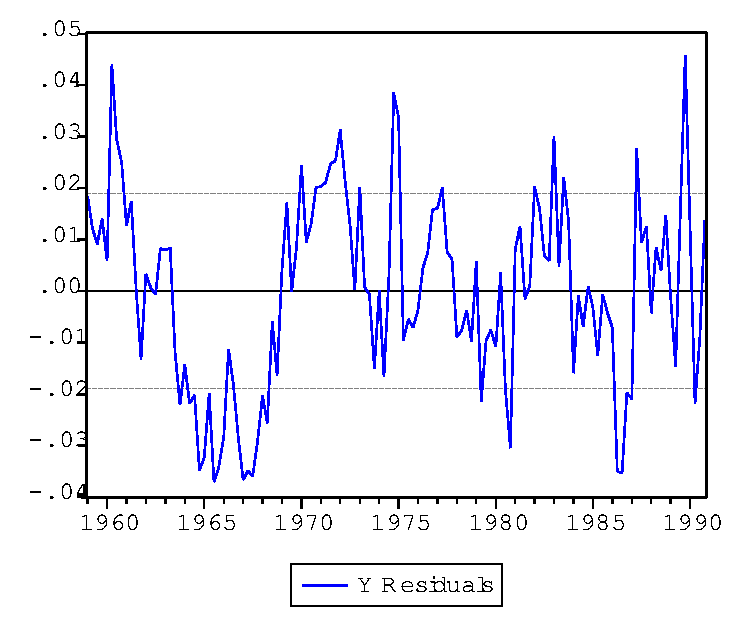
\includegraphics[scale=0.5,angle=0]{graph}
                    \caption{Estimated residuals from model XXX. ...}
                    \label{Fig:Resids}
                \end{center}
                \end{figure}

            \item Tables and graphics may appear in the text or in
                the appendix, especially if there are many simulation results
                tabulated, but is also depends on the study and number of tables resp.
                figures. The key graphs and tables must appear in
                the text!
        \end{itemize}

    \item Latex is really good at rendering formulas:\\
        {\it Equation (\ref{Eq:SpecDens}) represents the ACs of a stationary
        stochastic process:
        \begin{equation}
            f_y(\lambda) = (2\pi)^{-1} \sum_{j=-\infty}^{\infty}
                           \gamma_j e^{-i\lambda j}
                         =(2\pi)^{-1}\left(\gamma_0 + 2 \sum_{j=1}^{\infty}
        \gamma_j \cos(\lambda j)\right)
                                        \label{Eq:SpecDens}
        \end{equation}
        where $i=\sqrt{-1}$ is the imaginary unit, $\lambda \in [-\pi,
        \pi]$ is the frequency and the $\gamma_j$ are the autocovariances
        of $y_t$.}

\newpage

    \item Discuss results:
        \begin{itemize}
            \item Do the results support or do they contradict economic theory ?
            \item What does the reader learn from the results?
            \item Try to give an intuition for your results.
            \item Provide robustness checks.
            \item Compare to previous research.
        \end{itemize}
\end{itemize}

\section{Conclusions}\label{Sec:Conc}

\begin{itemize}

    \item Give a short summary of what has been done and what has been
    found.

    \item Expose results concisely.

    \item Draw conclusions about the problem studied. What are the
    implications of your findings?

    \item Point out some limitations of study (assist reader in judging validity
    of findings).

    \item Suggest issues for future research.

\end{itemize}




% ----------------
% --- appendix ---
% ----------------
\appendix

% literature
\newpage
\addcontentsline{toc}{section}{References}
\bibliography{literature}

% figures (not mandatory)
%\newpage
%\section{Figures}

\begin{figure}[ht]
    \begin{center}
        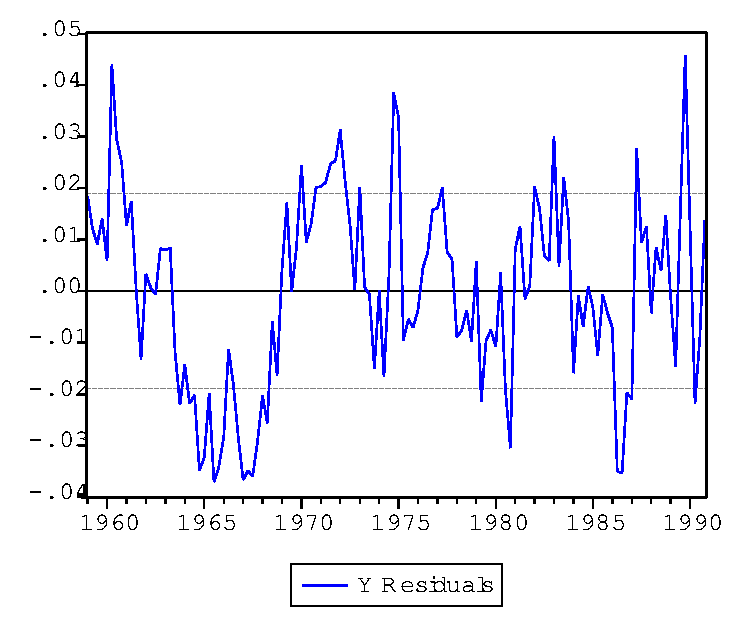
\includegraphics[scale=0.5,angle=0]{graph}
        \caption{Estimated residuals (2) from model XXX. ...}
        \label{Fig:Resids2}
    \end{center}
\end{figure}


% tables (not mandatory)
%\newpage
%\section{Tables}

\begin{table}[ht]
    \begin{center}
        {\footnotesize
        \begin{tabular}{l|cccccccccc}
        \hline \hline
                        & 3m    & 6m    & 1yr   & 2yr   & 3yr   & 5yr   & 7yr   & 10yr  & 12yr  & 15yr   \\
            \hline
                Mean   & 3.138 & 3.191 & 3.307 & 3.544 & 3.756 & 4.093 & 4.354 & 4.621 & 4.741 & 4.878  \\
                Median & 3.013 & 3.109 & 3.228 & 3.490 & 3.680 & 3.906 & 4.117 & 4.420 & 4.575 & 4.759  \\
                Min    & 1.984 & 1.950 & 1.956 & 2.010 & 2.240 & 2.615 & 2.850 & 3.120 & 3.250 & 3.395  \\
                Max    & 5.211 & 5.274 & 5.415 & 5.583 & 5.698 & 5.805 & 5.900 & 6.031 & 6.150 & 6.295  \\
                StD    & 0.915 & 0.919 & 0.935 & 0.910 & 0.876 & 0.825 & 0.803 & 0.776 & 0.768 & 0.762  \\
            \hline \hline
        \end{tabular}}
    \end{center}
    \caption{Detailed descriptive statistics of location and dispersion for
    2100 observed swap rates for the period from
    February 15, 1999 to March 2, 2007. Swap rates measured as 3.12 (instead of 0.0312).}
    \label{Tab:DescripStatsRawDataDetail}
\end{table}




% --------------------------------------------
% --- last page: Declaration of Authorship ---
% --------------------------------------------

%\newpage
%\thispagestyle{empty}
%%{\Large{\bf Declaration of Authorship}}\vspace{0.5cm}

\section*{Declaration of Authorship}

I hereby confirm that I have authored this Bachelor's/Master's
thesis independently and without use of others than the indicated
sources. All passages which are literally or in general matter
taken out of publications or other sources are marked as such.
\vspace{1cm}

Berlin, September 30, 2007 \vspace{0.5cm}

your name (and signature, of course)



\end{document}
